%===================================== CHAP 4 =================================

\chapter{Research Design and Methodology}
Over the course of this project, both quantitative and qualitative data gathering and analysis methods were employed. Both of the methods offered something valuable to the project, and using both allowed for gathering the data best suited for the thesis. In the early stages quantitative data, such as questionnaires, were used to gather opinions and thoughts from potential users of the program. Using these surveys, a base could be created to build from, and develop a better prototype. With this prototype finished, more qualitative measures were used to gather more specific and more detailed data. Figure \ref{fig:researchMethod} provided an overview of the research process applied in this thesis, from the strategy, data generation methods and data analysis methods.  

\begin{figure}[!ht]
     \centering
     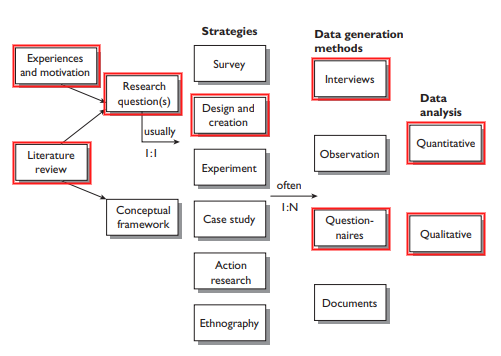
\includegraphics[width=.8\textwidth]{./fig/researchMethodology/OatesResearch.png}
     \captionsetup{width=0.8\linewidth}
     \caption{Model of the research process adapted from Oates \cite{oates2005researching}. The red outlined boxes are methods used in this thesis.}
     \label{fig:researchMethod}
 \end{figure}

\section{Design and Creation Research}
\label{sec:designCreationResearch}
One of the more common research methodologies in computer science, Design and Creation Research uses common development techniques and adapts them for research and is also the research methodology that will be used for this thesis. It focuses on development of new IT products, also called artefacts \cite{oates2005researching}. In the case of this paper, the artefact being developed is a prototype aiming to investigate whether or not collaboration is conducive to career guidance in virtual reality. This type of research can be split into a few different types, mostly depending on whether the artefact itself is the end goal, a vehicle for research or if the focus is on the development process itself. The most relevant case for this project is the second case. To expand upon this slightly, to say that the artefact is a vehicle for the research means that while the artefact itself is important, its \textit{usage} in real life is what's really important. By developing something that can be used in real life, it is possible to point to something concrete and measure the perceived effects the artefact has on the system it is introduced to.

While the artefact in this project is a vehicle for the research, the aim is to have one of the pre-existing workplace applications working with collaborative elements at close to 100\% functionality, so that others may continue developing the application later with relative ease. The most important part is still to see whether or not the end product can heighten the efficacy of the VR career guidance project.


\section{Development methodology}
The primary type of development used in the project can best be described as a variant of agile software development. Agile development refers to certain principles that were written down in the 2001 article \textit{Manifesto for Agile Software Development}\cite{beck2001manifesto}. This manifesto decries the old method of rigid development that was very resistant to change. Over the course of this project, feedback is sought at every level, hoping to improve the software both for the customer and the users, and that means that it must be open to change when it needs to.

There will be multiple iterations and phases of the project, each building upon the last. Three major phases were roughly planned out at the beginning of the project, with each containing multiple iterations as priorities shift based on feedback. These three phases are discussed in more detail in chapters \ref{chap:phase1}, \ref{chap:phase2} and \ref{chap:phase3}, respectively. Figure \ref{fig:devMethod} outlines the adapted develop methodology.

\begin{figure}[H]
     \centering
     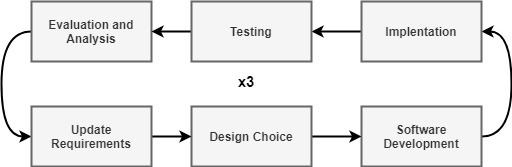
\includegraphics[width=.8\textwidth]{fig/researchMethodology/devMethod.jpg}
     \captionsetup{width=0.8\linewidth}
     \caption{The development methodology used in this thesis.}
     \label{fig:devMethod}
 \end{figure}



\section{Methods to Answer Research Questions}
The primary goal of the paper is to answer the research questions as posed by us. To do that, it's important that there is a clear and structured way to answer them. As the matters they pertain to vary to some degree, so too will the ways to answer them. 

First and foremost is the primary research question: "How does collaboration in virtual reality (VR) workplaces contribute to the career guidance of young job seekers?"  This RQ, along with secondary RQ1 and RQ2, will be answered mostly through traditional data gathering and analysis methods, i.e., surveys, user tests and expert tests. They're multi-faceted questions that need to be looked at from multiple angles, and as such, need multiple runs of data gathering to properly answer. Primarily, this will include user testing and interviews, with a side of surveys and focus groups.

Secondary RQ3 and RQ4, are more technical questions, and will be answered with the information gleaned from the design and creation method. Users are less involved with this, as it pertains more to the process of development and the interests of the IMTEL group as well as NAV. The process of development, needs and requirement will therefore be well documented to enable a comprehensive report as to the conversion process from single user experience to multi user experience. 



\section{User testing}
User tests are an important part of agile development. They are one of the primary means of gathering relevant feedback from the people who will actually be using your product. In essence, a user test is way to test the opinions of users who have had a chance to try the artefact being created. By employing user tests, it's possible to glean more unbiased information from users that do not have knowledge of the artefact or preconceived notions of its quality. A common pitfall when evaluating systems is letting your own knowledge of quirks and the intent, rather than the performance, of a functionality cloud your evaluation. With user testing, you can figure out what a mechanic looks like to those the artefact is intended for, gather data and make the proper adjustments to increase the value of the system.

A lot of care goes into creating the tests and making sure that the data extracted from them is sound and valid. The tests needs to specific enough to showcase or test the aspect you are focusing on, but not so specific that it becomes an unnatural situation that does not represent the actual product.


Most of the tests performed with the target audience has been done in collaboration with NAV. With their help, testers in the target group were gathered, and they could then try out the application collaboratively. The experience would be supervised by us, ready to guide or help if they struggled with the basic VR interactions, as the testers had quite varying levels of familiarity with VR. Once they had finished the tasks that were available to them they were asked questions through a semi-structured interview that had been planned out in advance.


\subsection{The Surveys}
The purpose of a survey is to obtain the same data from a large amount of people in a systematic way, and then analyse the data, looking for patterns to generalise to the larger population\cite{oates2005researching}. People often associate surveys with questionnaires, but a survey can consist of many other forms of data gathering. This project has opted to use several of these to be able adapt to the multiple situations. 

For surveys, it is important to reach a minimum desired response rate to ensure that you have a large enough sample size. In those situations where we opt to use quantitative data, steps should be taken to increase the response rate where possible. Since the plan is to conduct most of the primary data gathering in person, the response rate will hopefully be quite high. In the situations where we can not gather data in person, questionnaires may be employed instead. For those cases, it's possible to emphasise the importance of the project and thoroughly explain what we hope to achieve in an attempt to appeal to the responder's solidarity and curiosity. 

One of the most important parts of research is gathering the data. Often a choice must be made to go for either a smaller quantity of high quality data, i.e., qualitative data, or a larger selection of data points at the cost of the quality, i.e., quantitative data. There are merits to using both, and they will each suit different situations.

\subsubsection{Quantitative Data}
When shaping the surveys to gather quantitative data, it's necessary to shape the questions accordingly. The way you allow the respondent to answer will also shape your data. If the survey consists mostly of open questions, where the respondent can answer what they want to you may gain a a more detailed answer, but the respondent may also be less likely to answer it at all, as you've raised the barrier to answering\citep[p.~223]{oates2005researching}. Narrow down the possible answers too much, and the respondent may not find an answer they agree with. One of the more common formats for answers called is the Likert scale, after psychologist Rensis Likert\cite{likert1932technique}. It is designed to capture the degree of agreement or disagreement of the respondent, and strikes a middle ground between a simple yes/no question and an open one. Likert items are employed heavily in our surveys.


\subsubsection{Qualitative Data}
When quantitative data does not quite cover what you need, qualitative data can instead be of use. Sacrificing the possibility of a larger selection of feedback, one can then dig deeper for the answers you seek, as well as open up the possibility for a dialogue with the correspondents, in the case of a focus group or similar situations. To take proper advantage of the qualitative data gathered, some work is required to make it usable. This can take on different forms, but a common version is thematic analysis, where responses are checked for recurring keywords and themes, and categorised accordingly.

\subsubsection{Exploratory Work}
In the beginning phases of the project, it was deemed important to get an overview of the general attitude of the target audience when it came to VR. As such, plans were made to conduct quantitative data surveys of different parts of the target audience. This included both young job seekers, as well as NAV employees. For the first group, the most significant knowledge to be gained was what young job seekers felt was helpful and what was not when it came to VR. The previously developed applications at the IMTEL lab suited that purpose excellently and could be used to convey the possibilities as well as the limitations of VR, and hopefully evoke useful feedback.

For the second group, NAV employees, it was important to figure out how they usually worked with the job seekers. What did their workflow look like before, and how could the artefact of this project fit into that?


\subsection{Expert Evaluations}
Since most of the work of this project was done at the IMTEL lab, opportunities presented themselves for us to gather feedback and advice. Throughout the year, people from multiple fields and disciplines stopped by the lab for various reasons, and most were quite open to some discussion about the project. The multidisciplinary nature of the project meant that even if they were not necessarily well versed in every aspect, they still had some valuable input for us to consider.

Using the contacts of the lab managers, it was also possible to arrange larger scale information gathering sessions, where the application was demonstrated to people working in the field of career guidance and lifelong learning. Following the demonstration, a discussion was held, questions from the audience were fielded, and the participants were asked to answer a survey regarding the application. 

By doing this, we hoped to gather many different points of view in an effort to ensure that the product was interesting and valuable to use for all users.

\section{Data Gathering Schedule}
Table \ref{table:dataGatheringSchedule} shows the data gathering schedule of all dates where tests where performed and what methods was used. 
 
\begin{table}[H]
\centering
\begin{tabular}{l|l|l}
\toprule
{\textbf{Date}} & { \textbf{Place}} & { \textbf{Method}} \\ 
\midrule
27.09.2019   & NTNU Gløshaugen  &  Questionnaire                \\ 
04.11.2019  & NTNU Dragvoll & Expert feedback                   \\
25.11.2019   & NAV Falkenborg &  Interviews                     \\ 
09.03.2020  & NTNU Dragvoll &  Group discussion / questionnaires\\ 
21.04.2020   & Video conference &  Questionnaire                \\ 
24.04.2020   & Video conference &  Questionnaire                \\ 
14-24.05.2020   & Video conference &  Interviews                \\ 
\bottomrule
\end{tabular}
\caption{Data gathering schedule.}
\label{table:dataGatheringSchedule}
\end{table}


\cleardoublepage